\section{Návrh uživatelského rozhraní - HiFi prototyp}

Dalším krokem návrhu uživatelského rozhraní byla tvorba HiFi prototypu, neboli aplikace, která je již vytvořena za použití některých technologií cílové platformy, avšak neobsahuje backend - neukládá žádná data a vždy zobrazuje pouze předpřipravený obsah - vždy však musí správně reagovat na interakci uživatele.\\
Hi-fi prototyp jsme opět realizovali jako tým v rámci předmětu MI-NUR, avšak přípravu technologie jsem provedl já samostatně a její realizace stojí za zmínku.

\subsection{Technologie použitá v Hi-Fi prototypu}

Cílem bylo vytvořit jakýsi mikro-framework, ve kterém bude snadné tvořit Hi-Fi prototyp, a současně bude možné používat standardní prvky Material designu. Kód měl být psán v jazyku cílové platformy, tedy HTML + CSS + JS.\\
Jelikož nikdo z nás neměl zkušenosti s žádným z Javascriptových frameworků typu Angular či React, a chtěl jsem pro naše řešení mít co nejméně závislostí, rozhodl jsem se vše napsat v čistém Javascriptu (pouze za použití dnes de-facto standardní knihovny jQuery). Základem je jeden výchozí HTML soubor, viz ukázka kódu \ref{code:hifi-html}.

\begin{listing}[H]
\begin{minted}[linenos,frame=lines]{html}
<!DOCTYPE html>
<html>
<head>
  <title>SYSEL</title>

  <meta name="viewport" content="width=device-width, initial-scale=1.0">
  <meta charset="UTF-8">

  <!-- Material components all-in-one -->
  <link rel="stylesheet" type="text/css" href="https://unpkg.com/
  material-components-web@latest/dist/material-components-web.min.css"/>
</head>
<body>
  <div id="main-content" class="homepage-include"></div>

  <!-- Material design -->
  <script src="https://unpkg.com/material-components-web@latest/dist/
  material-components-web.min.js"></script>
  <!-- jQuery-->
  <script src="https://cdnjs.cloudflare.com/ajax/libs/jquery/
  2.2.4/jquery.min.js"></script>
  <!-- Custom scripts -->
  <script src="js/main.js"></script>
</body>
</html>
\end{minted}
\caption{Základní soubor index.html pro Hi-Fi prototyp} \label{code:hifi-html}
\end{listing}

Veškerý ostatní obsah je \emph{komponenta}, což je HTML šablona, která může být libovolně vkládána do jiných šablon, několikrát vedle sebe apod. Postupně jsem umožnil komponenty libovolně parametrizovat a samozřejmě je mezi sebou vyměňovat - například přechod na zcela jinou stránku je realizován přes \emph{výměnu komponenty}, která se zobrazuje v \code{\#main-content} v ukázce kódu \ref{code:hifi-html}.\\
Toto vše je možné díky pouhým 67 řádkům JS kódu. Úryvek je vidět v ukázce kódu \ref{code:hifi-js}.

\begin{listing}[H]
\begin{minted}[linenos,frame=lines]{javascript}
function loadDynamicContent(selector = '[class$="-include"]', callback){

  $(selector).each(function (e) {
    // load all custom components
    let parent = $(this);
    $(this).html('');
    $(this).load("components/" + $(this).attr("class")
      .replace("-include", "") +  ".html", function() {

      // load sub-components
      $(is).find('[class$="-include"]').each(function() {
        loadDynamicContent(this, function(){
            insertParameters(parent)
        });
      });
      if ($(this).find('[class$="-include"]').length === 0) {
        insertParameters(parent);
      }
      callback(this);
    });
  });
}

function insertParameters(parent) {
    let parameters = parent.attr('data-include-content');
    if (parameters !== undefined) {
        $.each(JSON.parse(parameters), function(key, value){
            parent.html(parent.html().replace('{' + key + '}', value));
        }
    }
}
\end{minted}
\caption{Funkce pro načtení obsahu komponent Hi-Fi prototypu, včetně podkomponent} \label{code:hifi-js}
\end{listing}

Funkce \code{loadDynamicContent} z ukázky kódu \ref{code:hifi-js} funguje tak, že projde existující kód (výchozí je vždy \code{index.html} z ukázky kódu \ref{code:hifi-html}) a veškeré výskyty tříd \code{něco-include} se snaží nahradit obsahem souboru \code{něco.html} ze složky \code{components/}. Díky tomu, že Javascriptu může být umožněn přístup na filesystém, lze takto dynamicky načítat obsah souborů z disku a renderovat ho přímo v již načteném obsahu. Tato technika je v některých browserech zablokována kvůli CORS\footnote{Cross-origin resource sharing - ochrana před načítáním nezabezpečeného obsahu}, a tak pro použití například v Google Chrome je nutné zmiňovaný \code{index.html} spouštět přes libovolný webserver, nelze jej přímo otevřít z filesystému. Naopak například v Mozilla Firefoxu je CORS v tomto ohledu volnějši, a celý tento mikro-framework tak lze používat bez jakéhokoliv lokálního serveru, stahování závislostí atp. - stačí pouze otevřit \code{index.html}.\\
Zdrojové kódy Hi-Fi prototypu, který následně v tomto \uv{frameworku} vznikl, jsou dostupné na přiloženém médiu a také v repozitáři na Gitlab FIT \cite{gitlab-hifi}. Stejně jako u Lo-Fi prototypu, i zde vkládám obrazovku naskladnění přímo do textu jako obrázek \ref{picture:hifi}.\\
Tento prototyp byl podroben uživatelskému testování, které je z důvodu logické struktury práce obsaženo v kapitole \ref{testing}, přestože chronologicky proběhlo ještě před dalšími návrhovými procesy, které budu popisovat v následujících sekcích.\\

\begin{figure}[]
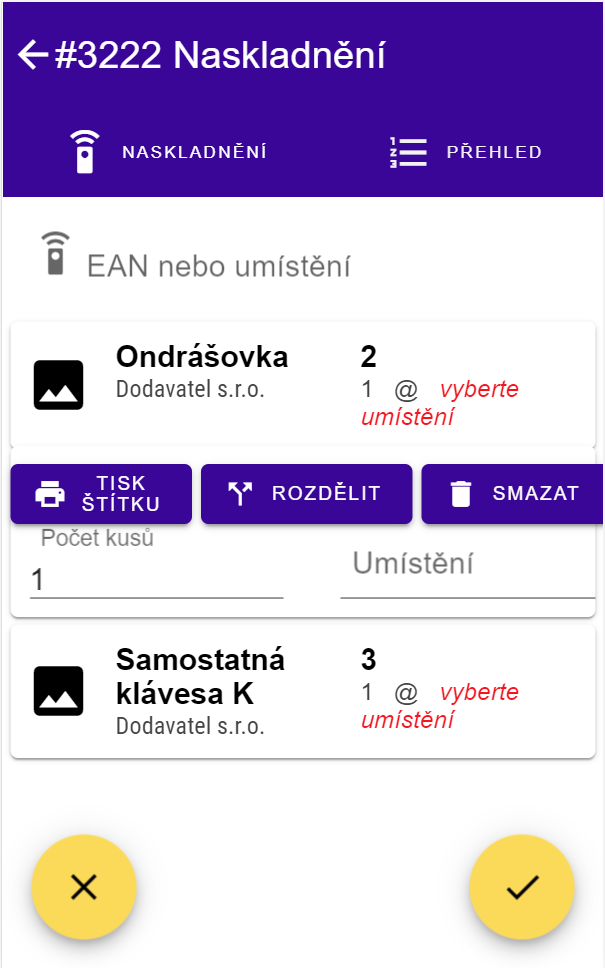
\includegraphics[height=0.6\textheight]{../png/hifi/naskladneni.png}
\caption{Rozhraní skladníka pro naskladňování položek: Hi-Fi prototyp} \label{picture:hifi}
\end{figure}
